\documentclass[a4paper, 10pt, fleqn]{article}
\usepackage{custom}
\usepackage{pageformatting}
\usepackage{tikz}
\usepackage{aeguill}
\usepackage{import}
\usepackage{pdfpages}

\usepackage[ngerman]{babel}
%mathe packages
\usepackage{amsmath}

%table packages
\usepackage{booktabs}
\newcommand{\tabitem}{~~\llap{\textbullet}~~}
\usepackage{tablefootnote}

\graphicspath{{sysspec/pdf/}{images/}{uml/}}

%============PAGE PROPERTIES=============
\newcommand{\revisiondate}{\today}
\newcommand{\documenttitle}{Clock Pendulum Analyzer} % used for title in title and subtitle pages
\newcommand{\authors}{Tobias Kreienbühl \& Daniel Föhn} %used for title page only
\newcommand{\subauthors}{im Auftrag der Hochschule Luzern} %used for title page only
\newcommand{\subtitle}{Projektdokumentation} % used for title and subtitle pages
\newcommand{\documentdesc}{Gesamtprojektdokumentation des \documenttitle}
\newcommand{\dozent}{Josef Bürgler}
\newcommand{\rpi}{Raspberry Pi 3}
\newcommand{\iic}{$I^2C$}
\newcommand{\hwb}{Hardware-Board}
\newcommand{\titleimage}{gesamtansicht.png}

\begin{document}
	\begin{titlepage}
		\titleGM
		\thispagestyle{empty}
	\end{titlepage}
	\clearpage
\thispagestyle{empty}
\section*{Selbständigkeitserklärung}
Die Verfasser bestätigen mit ihrer Unterschrift, dass die vorliegende Arbeit eigenständig und ohne fremde Hilfe oder Benutzung anderer als die angegebenen Hilfsmittel erstellt wurde.\\Sämtliche verwendeten Textausschnitte, Zitate oder Inhalte anderer Verfasser wurden ausdrücklich als solche gekennzeichnet.

\vspace{2cm}
\begin{tabular}{@{}l@{}}
    Rotkreuz, \today\\
    Ort, Datum
\end{tabular}
\vspace{10cm}

\begin{tabular}{@{}l@{}}\hline
    eigenhändige Unterschrift Tobias Kreienbühl
\end{tabular}
\vspace{2cm}

\begin{tabular}{@{}l@{}}\hline
    eigenhändige Unterschrift Daniel Föhn
\end{tabular}
\vspace{2cm}

\clearpage
    
	\tableofcontents
	
    %--- Management Summary ---
    \clearpage
    %!TEX root=Projektdokumentation_ClockPendulumAnalyzer.tex
\section{Management Summary}
	\clearpage
	\section{Einführung}
		\subsection{Zweck des Dokuments}
		\subsection{Zielpublikum}
		\subsection{Versionierung}
			\begin{table}[h]
				\centering
				\begin{tabularx}{\textwidth}{|c|c|X|}
				\hline
				\rowcolor{shadecolor}\textbf{Version} & \textbf{Datum} & \textbf{Kommentar}\\ \hline
				V1.0 & \today & initial file \\ \hline
				\end{tabularx}
			\end{table}
		\subsection{Glossar}
			\begin{description}
				\item[Abkürzung]- Erklärung
			\end{description}
    
    %--- Start of Vision ---
    \subtitlepage{Vision - Projektauftrag}
    \subimport{sysspec/}{vision.tex}
    
    %--- Start of PMP ---
    \subtitlepage{Projektmanagement}
    \subimport{pmp/}{projekt_organisation}
    \clearpage
    \subimport{pmp/}{projekt_rahmenplan}
    \clearpage
    %\subimport{pmp/}{zeitplanung}
    \clearpage
    \subimport{pmp/}{risiko}
    \clearpage
    \subimport{pmp/}{projekt_unterstutzung}
    \clearpage
    \subimport{pmp/}{testing}
    
    %--- Start of Sys Spec ---
    \subtitlepage{System Spezifikation}
    \subimport{sysspec/}{hardware}
    \clearpage
	\subimport{sysspec/}{systemdesign.tex}
    \clearpage
    \subimport{sysspec/}{interfaces.tex}
    
    %--- Fazit ---
    \clearpage
   	%!TEX root=Projektdokumentation_ClockPendulumAnalyzer.tex
\section{Ausblick}
Der vorliegende Prototyp eines \documenttitle\ bietet eine Grundlage, um diverse Arten von Uhrenpendel auf einige Mikrosekunden genau auszumessen. Die Genauigkeit ist hauptsächlich durch den Sensor und den Referenzkristall gegeben, die übrigen Systemelemente arbeiten konstant, dies bedeutet, der Zeitbedarf ist immer gleich und somit hebt sich dies zwischen zwei Messungen auf.\\
Das System kann somit mit den folgenden Massnahmen optimiert werden:
\begin{itemize}
	\item Ersatz des eingebauten Kristalls des tiny K20 Mikrocontroller-Boards durch einen externen, hochgenauen Kristall, z.B. einem NH25M22TA der Firma NDK. Mit einer Abweichung von 0.003ppm der 3ppb\footnote{Parts per Billion} und einer Spannung von 3.3V lässt er sich direkt an das tiny K20 anschliessen und würde auch im Gehäuse noch Platz finden. Nachteil ist der Stückpreis von ca. 85.- Franken bei einem Stück. Mit 10MHz eignet sich die Frequenz, um den Flankenzähler des tiny K20 zu speisen. Das Datenblatt befindet sich im Anhang ab Seite \pageref{app:NH25M22TA}.
	\item Verwenden eines anderen Sensors. Beispielsweise eine Laserschranke anstelle einer Infrarot-Schranke mit entsprechend weniger Streuung dank dem dünneren Laserstrahl. Allerdings konnte während der Recherchephase keine geeignete Laserschranke gefunden werden, welche keinen Empfänger benötigt.
	\item Einsatz eines leistungsstärkeren Mikrocontroller-Systems. Aktuell werden an der Hochschule Luzern Technik \& Architektur die ersten Modelle des neuen tiny K22 hergestellt. Dieses neue Board weist gegenüber dem kleineren K20 folgende Vorteile auf und ist ebenfalls für ca. 20.- Franken erhältlich (Abbildung \ref{fig:tinyk22-overview}, mcuoneclipse.com):
	\begin{itemize}
		\item 160Mhz Prozessor, Freescale K22
		\item 512 KByte FLASH und 128 KByte RAM.
		\item Grössere Anzahl I/O Ports.
		\item Eigener Freescale K20 Prozessor und USB Port zum Debuggen. 
	\end{itemize}
	Allerdings weist das tiny K22 andere Footer auf, so dass das \hwb\ entsprechend neu gestaltet werden müsste.
	\item Vollumfänglicher Einsatz der RTC zusammen mit dem GPS-Modul: Die RTC könnte als eigener Zeitgeber genutzt werden, wenn kein NTP-Server verfügbar ist. Die entsprechenden \iic Anschlüsse sind auf dem \hwb\ vorhanden. Mit Hilfe des GPS-Moduls kann die aktuelle Umgebungszeit über UART-RS232 gesetzt werden. Diese Anschlüsse sind ebenfalls bereits vorbereitet.  
\end{itemize}
\begin{figure}[H]
	\centering
	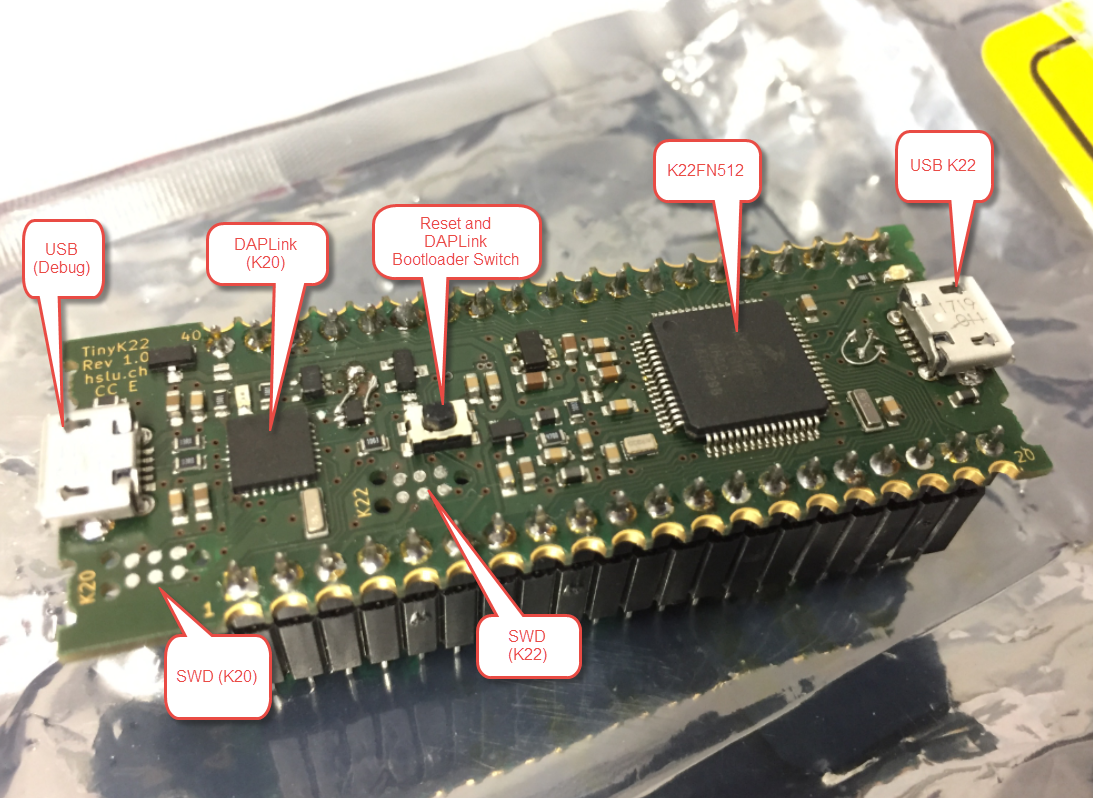
\includegraphics[width=0.5\textwidth]{tinyk22-overview}
	\caption{Tiny K22 Board mit eigenem Debug- Anschluss (Bildquelle: mcuoneclipse.com)}
	\label{fig:tinyk22-overview}
\end{figure}
Aktuell ist die Zähler-Frequenz von 12MHz in allen Softwareteilen fest eingetragen. Entsprechend müsste diese bei einer Änderung angepasst werden. Optimalerweise kann das System so erweitert werden, dass die Frequenz über ein Konfigurations-File eingestellt werden kann oder vom Mikrocontroller- System gleich automatisch ermittelt und gesetzt wird.\\
Allerdings bedingt der Einsatz eines externen Zählers ebenfalls Änderungen an der Software und es ist kaum anzunehmen, dass sich die Zählerfrequenz laufend ändert.
    %!TEX root=Projektdokumentation_ClockPendulumAnalyzer.tex
\section{Fazit}
Das vorliegende Projekt \documenttitle\ konnte weitgehend erfolgreich abgeschlossen werden. Die meisten Anforderungen und Resultate konnten erfüllt und erreicht werden. 
Der Vorliegende \documenttitle\ ermöglicht sowohl das Ausmessen von einfachen Pendeln, von Doppelpendeln und von Kreispendeln. Bei Doppelpendeln wird jeweils nur ein Pendel gemessen.\\
Durch die optischen Hilfsmittel wie der LED auf dem Sensor benötigt es nur wenig Kenntnisse, um das System erfolgreich nutzen zu können. Auch die benötigten Computerkenntnisse beschränken sich auf ein Minimum.\\
Das System lässt sich bei Bedarf erweitern und die Grösse des Gehäuses lässt auch noch Umbauten und das Anbringen von Erweiterungen zu. Sämtliche benötigten Anschlüsse sind eindeutig am Gehäuse angebracht, ein Verwechseln beim Anschliessen ist nicht möglich. Auch kann der Sensor nicht falsch angeschlossen werden. Einzig Arbeiten im Inneren des Gehäuses benötigen tiefere Systemkenntnisse.\\
Mittels der externen GPS Antenne kann eine stabile Verbindung erreicht werden.\\
\\
Nicht oder nur teilweise erreicht worden sind die folgenden Anforderungen:
\begin{itemize}
	\item Die Genauigkeit soll mit einer quadratischen Approximation erfolgen.\\
	Die quadratische Approximation dient der Berechnung der Pendelgeschwindigkeit. Es wären entsprechend drei oder mehr Sensoren notwendig gewesen, was aus Platzgründen schon sehr schwierig umzusetzen ist. Die Pendelgeschwindigkeit wird für die Messung zwischen zwei Ticks nicht benötigt. Deshalb ist diese Anforderung verworfen worden.
	\item Als Referenzclock soll für Prototyp 1 eine 32kHz RTC verwendet werden, für Prototyp 2 eine GPS-
disziplinierte 10MHz RTC.\\
	Es konnte mittels dem verwendeten 12MHz Kristall ein guter Kompromiss gefunden werden und das System lässt sich leicht mit einem hochgenauen Kristall optimieren, wie bereits im Ausblick beschrieben.
	\item (Optional) Es soll die Temperatur gemessen werden, um einen allfälligen Einfluss auf die Pendelge-
nauigkeit anzeigen zu können.\\
	Diese, optionale Anforderung wurde aus Zeitgründen weggelassen. Die verwendeten Hardware-Elemente lassen allerdings ein Nachrüsten zu.
	\item (Optional) Es soll die Luftfeuchtigkeit gemessen werden, um einen allfälligen Einfluss auf die Pen-
delgenauigkeit anzeigen zu können.\\
Analog zur Temperaturmessung.
	\item (Optional) Die Messgenauigkeit muss im Nanosekundenbereich liegen.\\
	Um die Genauigkeit im Nanosekundenbereich erreichen zu können muss das System mit einem hochgenauen Kristall getaktet werden.
\end{itemize}
Bei den Projektresultaten konnten ebenfalls nahezu alle Forderungen erreicht werden, einzig die Browserdarstellung konnte bis zum Abgabetermin der Dokumentation nicht fertiggestellt werden.\\
\\
Die Ursache der nicht erreichten Anforderungen und Resultate sind folgendermassen zu begründen:
\begin{itemize}
	\item Die Komplexität, insbesondere bei den elektronischen Bauteilen hat zu grösserem Zeitbedarf bei der Realisierung geführt, als gedacht. Bereits kurz nach Projektstart mussten die Entscheide Vorliegen, mit welchen Bauteilen das Projekt umgesetzt werden soll. Wie die Sensoren angeschlossen werden müssen und wie sich diese verhalten, musste von Grund auf erlernt werden und wäre ohne Unterstützung durch die Abteilung Elektrotechnik der Hochschule Luzern kaum zu bewältigen gewesen.
	\item Erfahrungen, welche Sensoren sich gut eignen würden und warum mussten ebenfalls erst gesammelt werden.
\end{itemize}

\clearpage
\subsection{Lessons learned}
	Aufgrund der häufigen Team-Besprechungen, die meistens eher kurz ausgefallen sind, konnten allfällige Konfliktpunkte und Schwierigkeiten schnell erkannt und unkompliziert behandelt werden. Aufgrund der Fehlenden Vorkenntnissen des Teams im Bereich der hochgenauen Kristalle und weiteren, hauptsächlich Elektronik-lastigen Themen musste vieles erst erlernt werden.\\
	Die Schwierigkeiten bei der Inbetriebnahme der elektronischen Bauteile und der Vorgehensweise bei der Auswertung von Zählern hat dann auch zu diversen Verzögerungen und Umorganisationen geführt. Dennoch konnte insgesamt stetig vorwärts gearbeitet und selten angefangene Arbeiten komplett verworfen werden. Einzig einige Sensoren haben die ersten Gehversuche, verbunden mit falschen Schaltungen nicht überstanden und mussten entsprechend nachbestellt werden.\\
	Um als Team erfolgreich zu sein, braucht es die Bereitschaft, sich auf einander zu verlassen, auf die Stärken jedes Teammitglieds zu Vertrauen und die Bereitschaft, sich Konflikten und Herausforderungen zu stellen, diese zu bewältigen und entsprechende Erfolge gemeinsam zu feiern.
	Das Team ist Stolz auf die geleistete Arbeit und das erstellte Produkt. Jeder konnte viele Erfahrungen sammeln.
		
    
    %BIBLIOGRAPHY
    \clearpage
    \nocite{*}
    \bibliography{bibliography}
    \bibliographystyle{apacite}
    
    %--- Start of Lists ---
    \clearpage
    \listoffigures
    \listoftables
    
    %--- Start of Appendix ---
    \clearpage
   	\section*{Anhang A - Sprint Reviews und Planung}
    \subimport{pmp/}{sprintplanning}
    
    \clearpage
    \section*{Anhang B - Arbeitsjournals}
    \newcommand{\header}{\textbf{Work Item}&\textbf{Datum}&\textbf{Zeitaufwand (in Std)}\\\toprule}
\newcommand{\footer}{\midrule\textbf{Total Arbeitsstunden}&-&\textbf{163.75}\\\midrule\bottomrule}
\begin{tabular}{ll}
    Entwickler: & Daniel Föhn \\
    Arbeitsperiode: & 18.09.2017 - 04.01.2018\\
\end{tabular}
\begin{longtable}{p{9cm}|p{2cm}|c}
    \header

    Administrativer Aufwand & 28.09 & 3\\
    & 05.10 & 2\\
    & 06.10 & 2\\
    & 19.10 & 1\\
    & 23.11 & 1.5\\
    & 30.11 & .5\\ 
    \hline
    
    Dokumentation & 05.10 & 2\\
    & 19.10 & 2.5\\
    & 02.11 & 5\\
    & 09.11 & 6\\
    & 14.11 & 0.5\\
    & 17.11 & 5\\
    & 22.11 & 3\\
    & 01.12 & 1\\
    & 07.12 & 7.5\\
    & 08.12 & 3\\
    & 14.12 & 4.5\\
    & 15.12 & 1\\
    & 17.12 & 0.75\\
    & 21.12 & 9.75\\
    & 28.12 & 5\\
    & 29.12 & 4\\
    & 03.01 & 5.5\\ 
    \hline
    
    Recherche Sensoren & 05.10 & 3\\
    \#3: Die Entwickler haben Zugriff auf PM und VCS& 28.09 & 1.5\\
    \#5: Der PO hat eine Grundstruktur des Projekt Reports& 28.09 & 2\\
    \#15: Der Projektreport hat einen Rahmenplan & 28.09 & 0.5\\
    & 29.09 & 1\\
    \#7: Das Projekt hat Risiken aufgeführt & 29.09 & 2\\
    \#28: Sensor Testaufbau & 06.10 & 2.25\\
    & 26.10 & 9\\
    & 27.10 & 2\\
    & 28.10 & 2\\
    & 01.11 & 2\\
    & 02.11 & 2\\
    \#38: Raspberry Pi aufsetzen & 19.10 & 1\\
    & 20.10 & 4\\
    \#27: Sensoren in Betrieb nehmen & 19.10 & 2\\
    \#24: Sensorwerte auf Display & 19.10 & 0.5\\
    \#45: Software zum Auswerten der Sensoren & 15.11 & 0.5\\
    & 16.11 & 2.5\\
    & 17.11 & 4\\
    & 02.01 & 4\\
    & 03.01 & 1\\
    Entwickeln der Kommunikation zwischen Counter und Rpi & 15.12 & 5.5\\
    & 30.12 & 2\\
    \#47: DB Software implementieren & 22.11 & 5\\
    & 23.11 & 4.5\\
    & 30.11 & 5.5\\
    & 01.12 & 3\\
    & 14.12 & 2.5\\
    \#50: REST Implementation & 02.01 & 3.5\\
    & 03.01 & 0.75\\
    & 04.01 & 6.75\\
    
    \footer
\end{longtable}

\noindent Es stehen noch einzelne Arbeitspakete aus, die nach Abgabe des Arbeitsjournal anfallen. Diese Aufgaben werden in der untenstehenden Auflistung geschätzt.\\
\\
Ausstehende Arbeiten:\\
\begin{tabular}{p{9cm}|c}
    \textbf{Work Item}     & \textbf{Zeitaufwand (in Std)} \\\hline
    Präsentation entwerfen & 8\\
    Projekt abschliessen   & 6\\
    anfallende Bug Fixes   & 2\\ \midrule
    \textbf{Total geschätzte Stunden} & \textbf{16}\\ \midrule\bottomrule
\end{tabular}
    \clearpage
    %\newcommand{\header}{\textbf{Work Item}&\textbf{Datum}&\textbf{Zeitaufwand (in Std)}\\\toprule}
%\newcommand{\footer}{\midrule\textbf{Total Arbeitsstunden}&-&\textbf{157.00}\\\midrule\bottomrule}
    \begin{tabular}{ll}
        Entwickler: & Tobias Kreienbühl \\
        Arbeitsperiode: & 18.09.2017 - 22.12.2017\\
    \end{tabular}

	\begin{longtable}{p{9cm}|p{2cm}|c}
		\header
		\textbf{Beschreibung} 	& \textbf{Datum} 	& \textbf{Zeitaufwand}\\
		Recherche Sensoren 		& 27.09.2017 		& 1h 30min\\\midrule
            Erstellen Grobkonzept 	& 28.09.2017 		& 3h 15min\\\midrule
            Erweiterung Grobkonzept & 01.10.2017 		& 4h\\\midrule
            Zwischenbesprechung und Planung Layout der Hardware	& 05.10.2017	& 5h\\\midrule
            Defintive Entscheidung Hardware		& 12.10.2017 & 4h\\\midrule
            Beschaffung Hardware und Material für Testgehäuse  & 14.10.2017 & 4h 15min \\\midrule
		Erstellen Testgehäuse  & 15.10.2017 & 4h\\\midrule
		Gemäss erster gedachter Schaltung, Erstellen eines Prototypenboardes für den Sensor & 18.10.2017 & 3h 30min\\ \midrule
		Annahme RTC und GPS-Modul & 19.10.2017 & 30min \\\midrule
		Versuch1: Sensor an Raspberry Pi anhängen und testen -> vermeindlicher Erfolg & 19.10.2017 & 4h 30min \\ \midrule
		Analyse Datenblätter und anlöten erster Pins zum Test der RTC und GPS & 26.10.2017 & 7h 30min\\ \midrule
		Beschaffen Logic-Analyser und kurze Instruktion & 26.10.2017 & 30min \\\midrule
		Weitere Recherche RTC & 28.10.2017 & 2h \\\midrule
		Auswerten RTC 32kHz Frequenz mit Hilfe Logic Analyser und Versuchsboard & 02.11.2017 & 5h 30min \\\midrule
		Recherche Hardware-Counter, Evaluieren von möglichen IC's & 02.11.2017 & 2h\\ \midrule
		Beschaffen eines TinyK20, anlöten Footer & 03.11.2017 & 3h 30min \\\midrule
		Inbetriebnahme TinyK20 mit Kinetis Design Studio und Debugger & 04.11.2017 & 3h \\ \midrule
		Verbinden und Testen GPS mit TinyK20, Sysnchonisation testen. & 9.11.2017 & 4h 30min\\\midrule
		Versuch, Sensor anzuhängen, fehlschlag & 16.11.2017 & 4h 30min\\\midrule
		Prototypen-Board mit Steckplätzen für GPS, RTC und Tiny erstellt & 22.11.2017 & 2h 30min \\ \midrule
		Weitere Versuche mit Sensor und Tiny, GPS-Verbindung mit Interrupt erfolgreich & 23.11.2017 & 5h 30min\\ \midrule
		Besprechung & 23.11.2017 & 30min \\ \midrule
		Layout PCB für Sensor nach erstem Schema & 27.11.2017 & 1h 30min \\\midrule
		Verbindungen fix auf Prototypen-Board anbringen & 29.11.2017 & 2h 30min \\\midrule	
		Ausbau Software für TinyK20 & 30.11.2017 & 4h 30min\\\midrule
		Entgegennehmen und Löten PCB's für Sensoren & 06.12.2017 & 2h 30min\\\midrule
		Dokumentation & 07.12.2017 & 8h 30min \\\midrule
		Dokumentation & 10.12.2017 & 6h 30min \\\midrule
		Ermitteln Fehler am Sensor & 13.12.2017 & 3h 30min\\\midrule
		Erstellen neues Schema, neues PCB in Auftrag geben & 13.12.2017 & 2h 30min\\\midrule
		Dokumentation & 14.12.2017 & 4h 30min\\\midrule
		Hardwareboard erweitern & 20.12.2017 & 5h 30min \\ \midrule
		Neues PCB bestücken und testen, Softwareerweiterung Mokrocontroller & 21.12.2017 & 9h 30min  \\ \midrule
		Steckeranschluss ändern und Kabelkonfektion & 22.12.2017 & 3h 30min  \\ \midrule
		Gehäusekonstruktion & 26.12.2017 & 6h  \\ \midrule
		Gehäusefertigung & 27.12.2017 & 8h 30min  \\ \midrule
		Gehäusefertigung & 28.12.2017 & 3h 30min  \\ \midrule
		Anschlüsse für Bauteile am Gehäuse, neues PCB für Sensor bestücken und testen. Gesamttest Hardware & 29.12.2017 & 7h 45min  \\ \midrule
		Gehäuse fertig montieren, lackieren, auskleiden, ölen & 30.12.2017 & 6h 30min  \\ \midrule
		Montage der elektronischen Bauteile im Gehäuse, Test der Hardware, Auskleiden mit Schallschutz & 31.12.2017 & 5h \\ \midrule
		Systemtest mit Uhr, Dokumentation & 02.01.2018 & 8h 30min \\ \midrule
		Dokumentation & 03.01.2018 & 4h 30min \\ \midrule
		Dokumentation & 04.01.2018 & 6h 45min \\ \midrule
		Dokumentation & 05.01.2018 & 4h \\ \midrule
		%TOTAL 			
		\textbf{Total Arbeitsstunden}
		&
            -
            &
		\textbf{194h}\\\midrule\bottomrule
	\end{longtable}

\clearpage
\noindent Es stehen noch einzelne Arbeitspakete aus, die nach Abgabe des Arbeitsjournal anfallen. Diese Aufgaben werden in der untenstehenden Auflistung geschätzt.\\
\\
Ausstehende Arbeiten:\\
\begin{tabular}{p{9cm}|c}
    \textbf{Work Item}     & \textbf{Zeitaufwand (in Std)} \\\hline
    Präsentation entwerfen & 8\\
    Präsentation vorbereiten & 8 \\
    anfallende Bug Fixes   & 2\\ \midrule
    \textbf{Total geschätzte Stunden} & \textbf{18}\\ \midrule\bottomrule
\end{tabular}
    
    \clearpage
    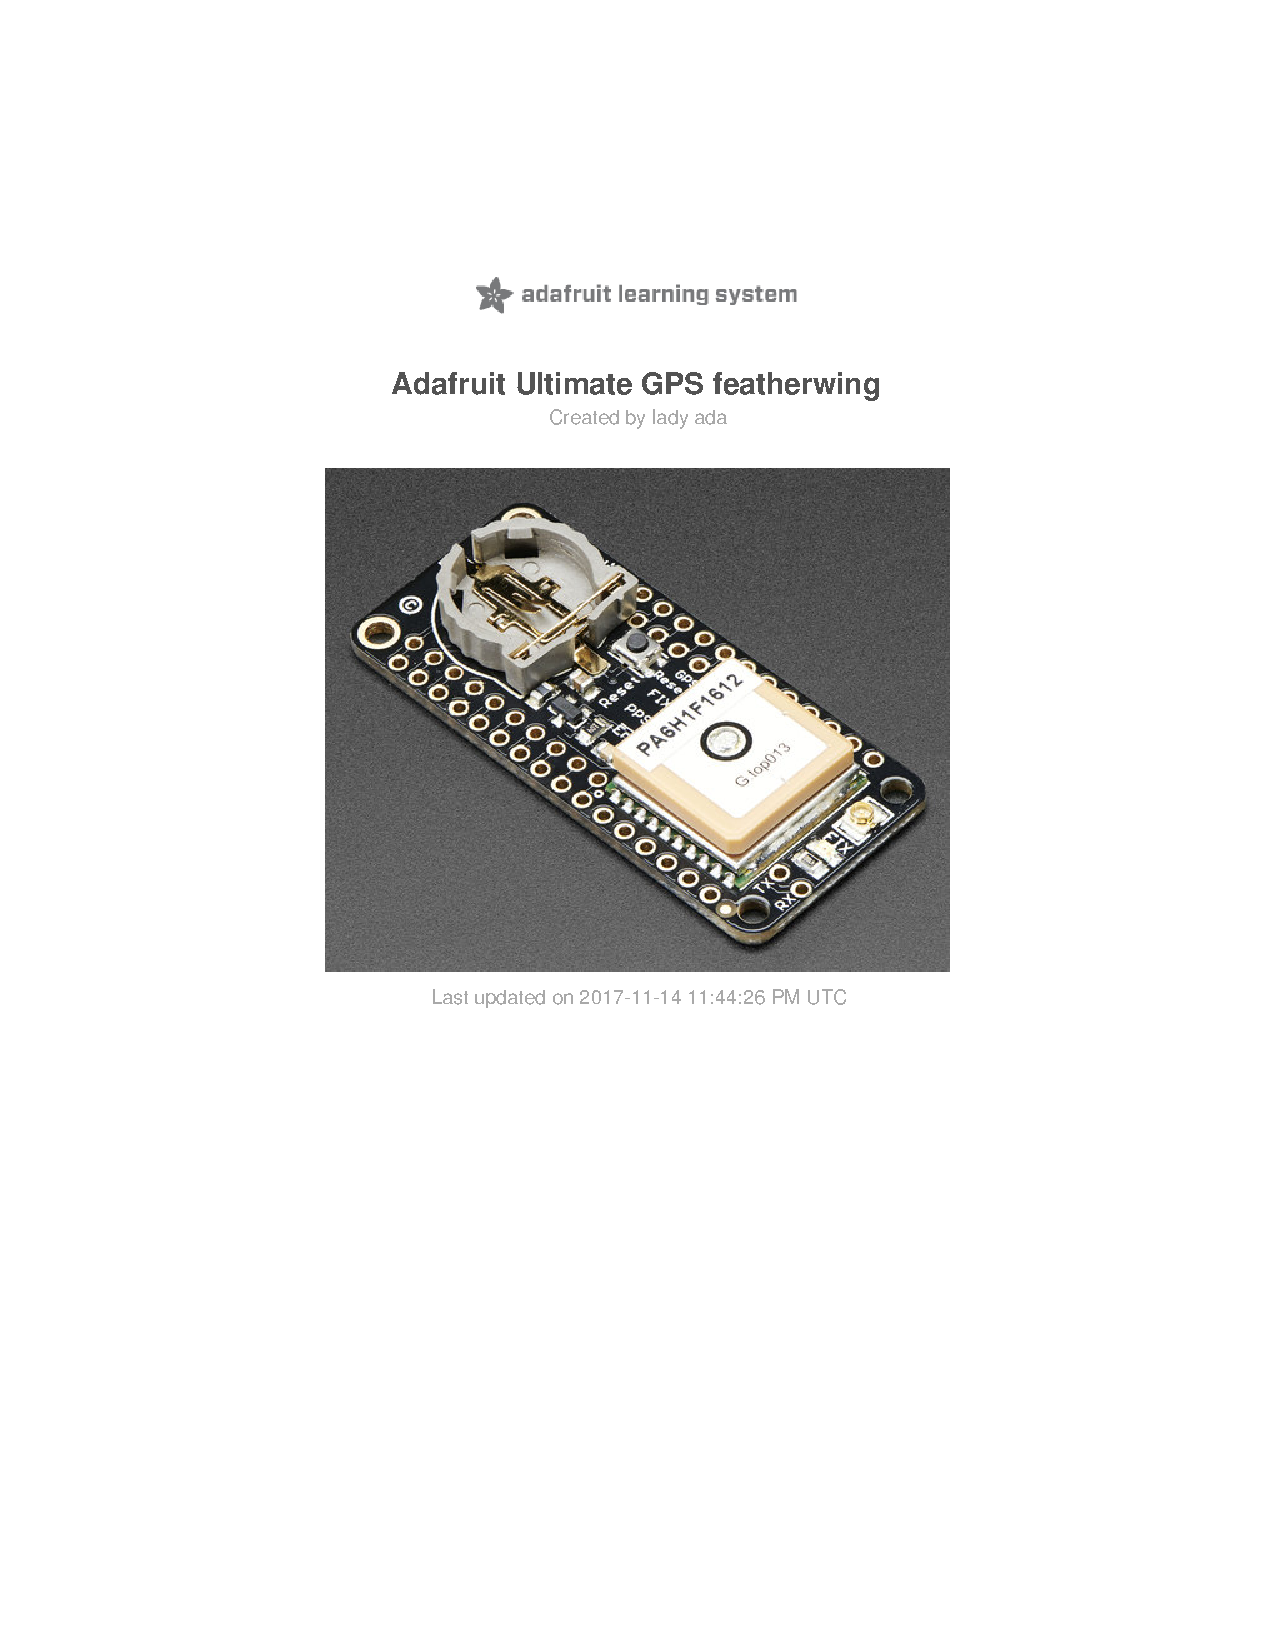
\includepdf[pages=1,pagecommand={\section*{Anhang C - Data Sheets}\subsection*{Adafruit Featherwing}\label{app:adafruit}},scale=0.8,frame=true]{adafruit-ultimate-gps-featherwing.pdf}
    \includepdf[pages={2-},scale=0.8,frame=true]{adafruit-ultimate-gps-featherwing.pdf}
    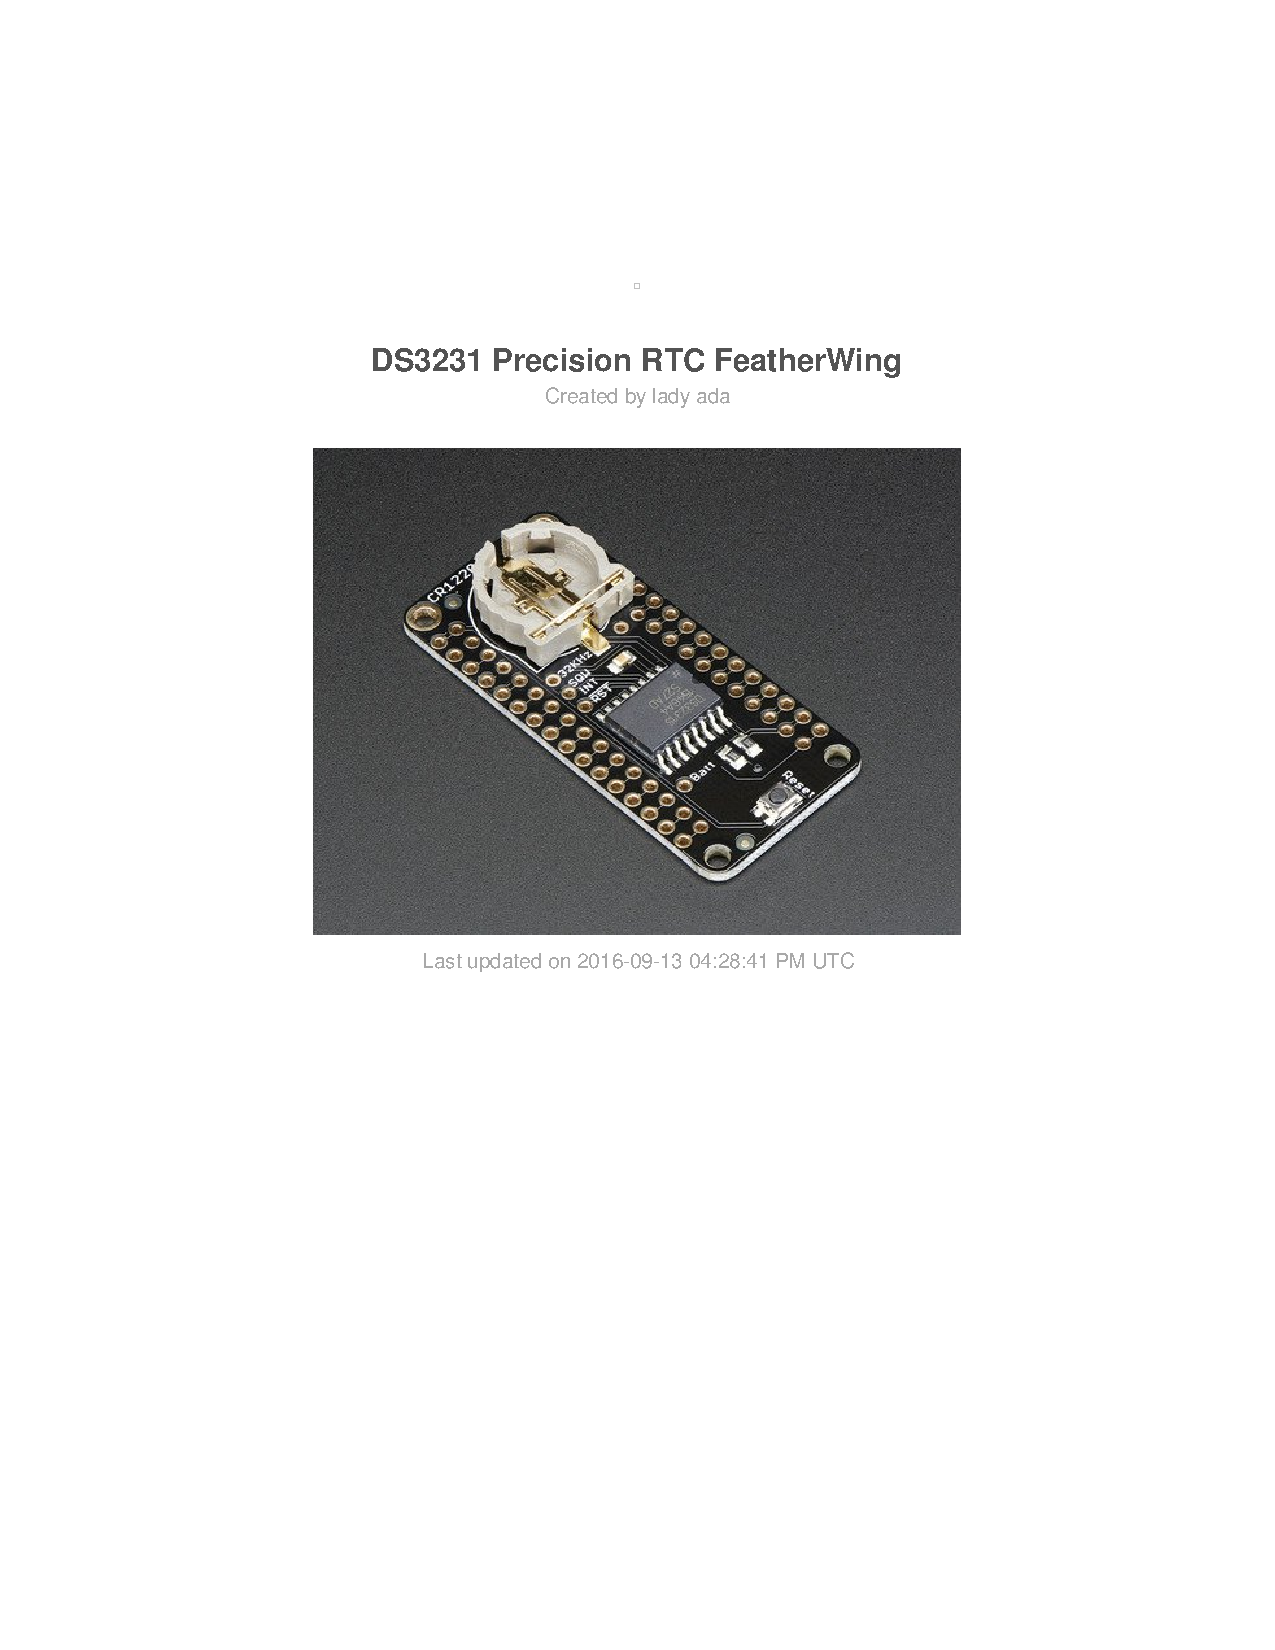
\includepdf[pages={1},pagecommand={\subsection*{Precision RTC Featherwing}\label{app:rtc_featherwing}},scale=0.8,frame=true]{ds3231-precision-rtc-featherwing.pdf}
    \includepdf[pages={2-},scale=0.8,frame=true]{ds3231-precision-rtc-featherwing.pdf}
    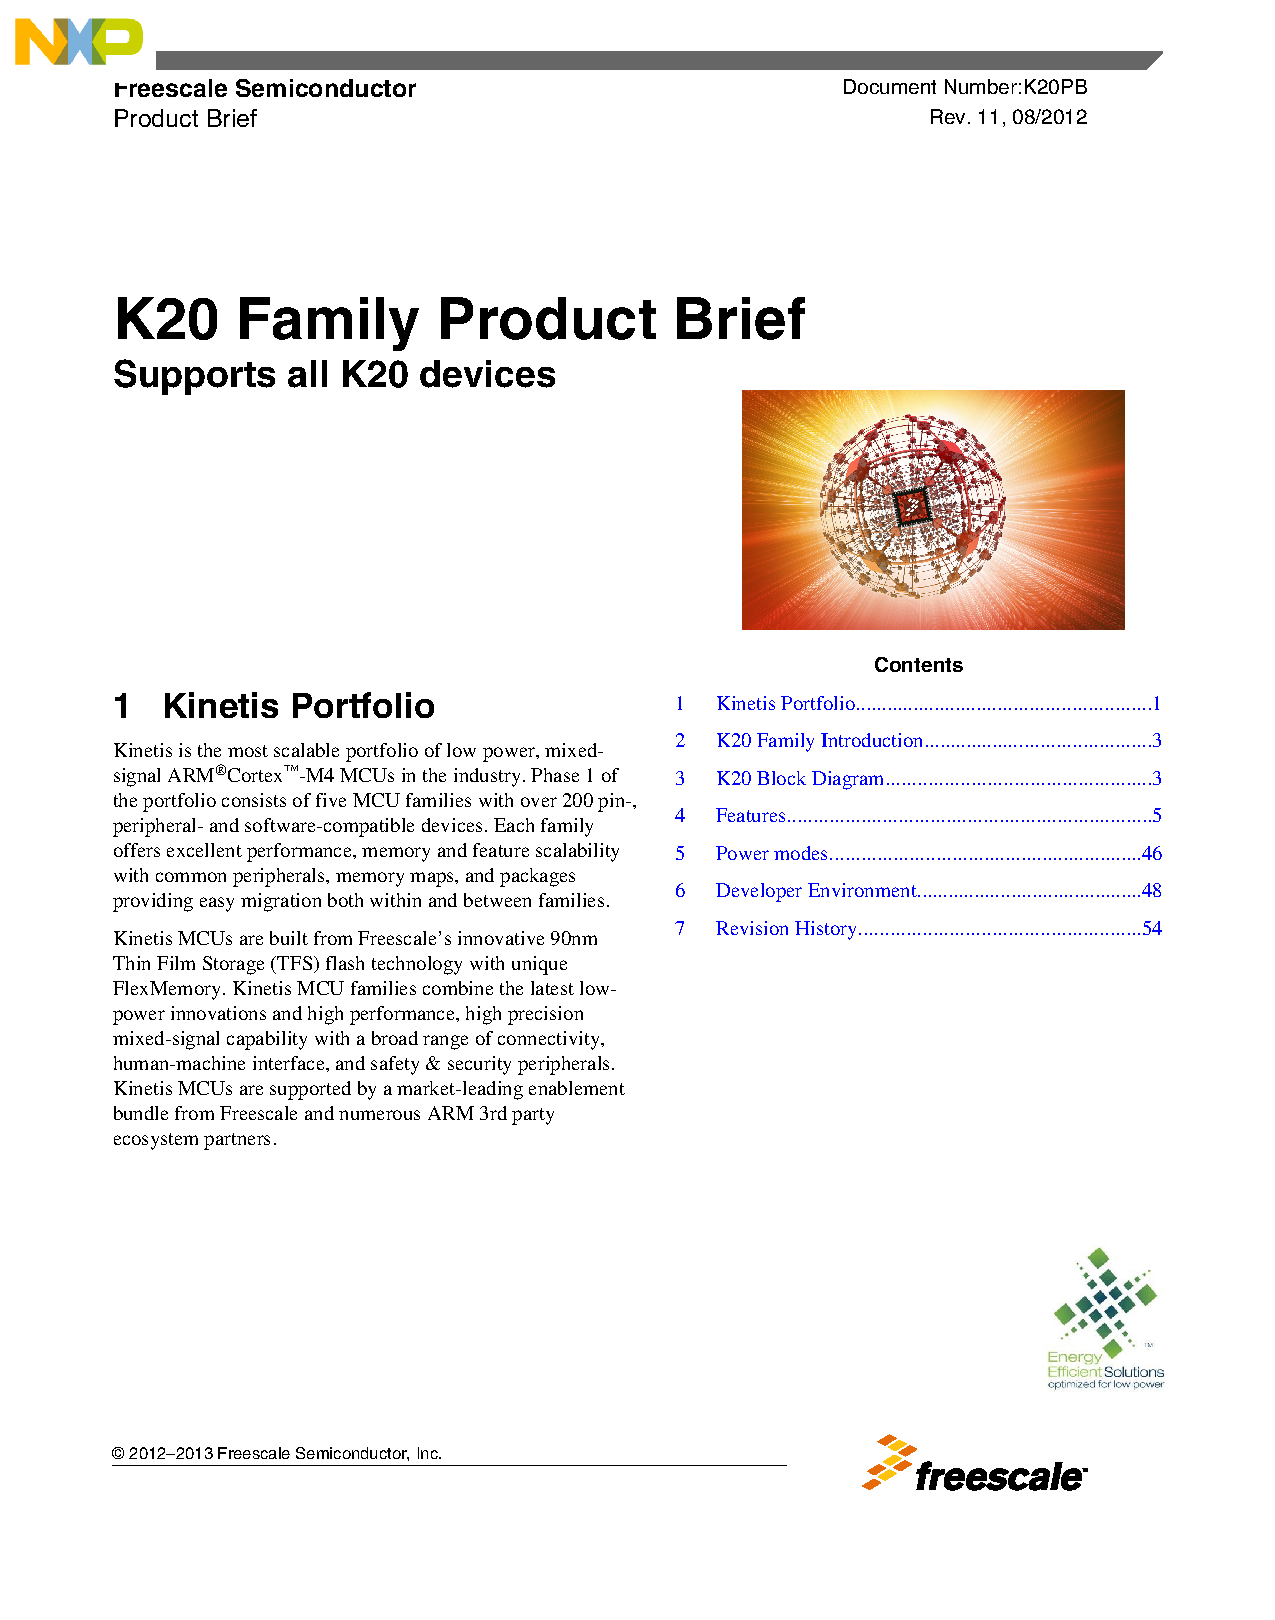
\includepdf[pages={1},pagecommand={\subsection*{K20PB}\label{app:K20PB}},scale=0.8,frame=true]{K20PB.pdf}
    \includepdf[pages={2-},scale=0.8,frame=true]{K20PB.pdf}
    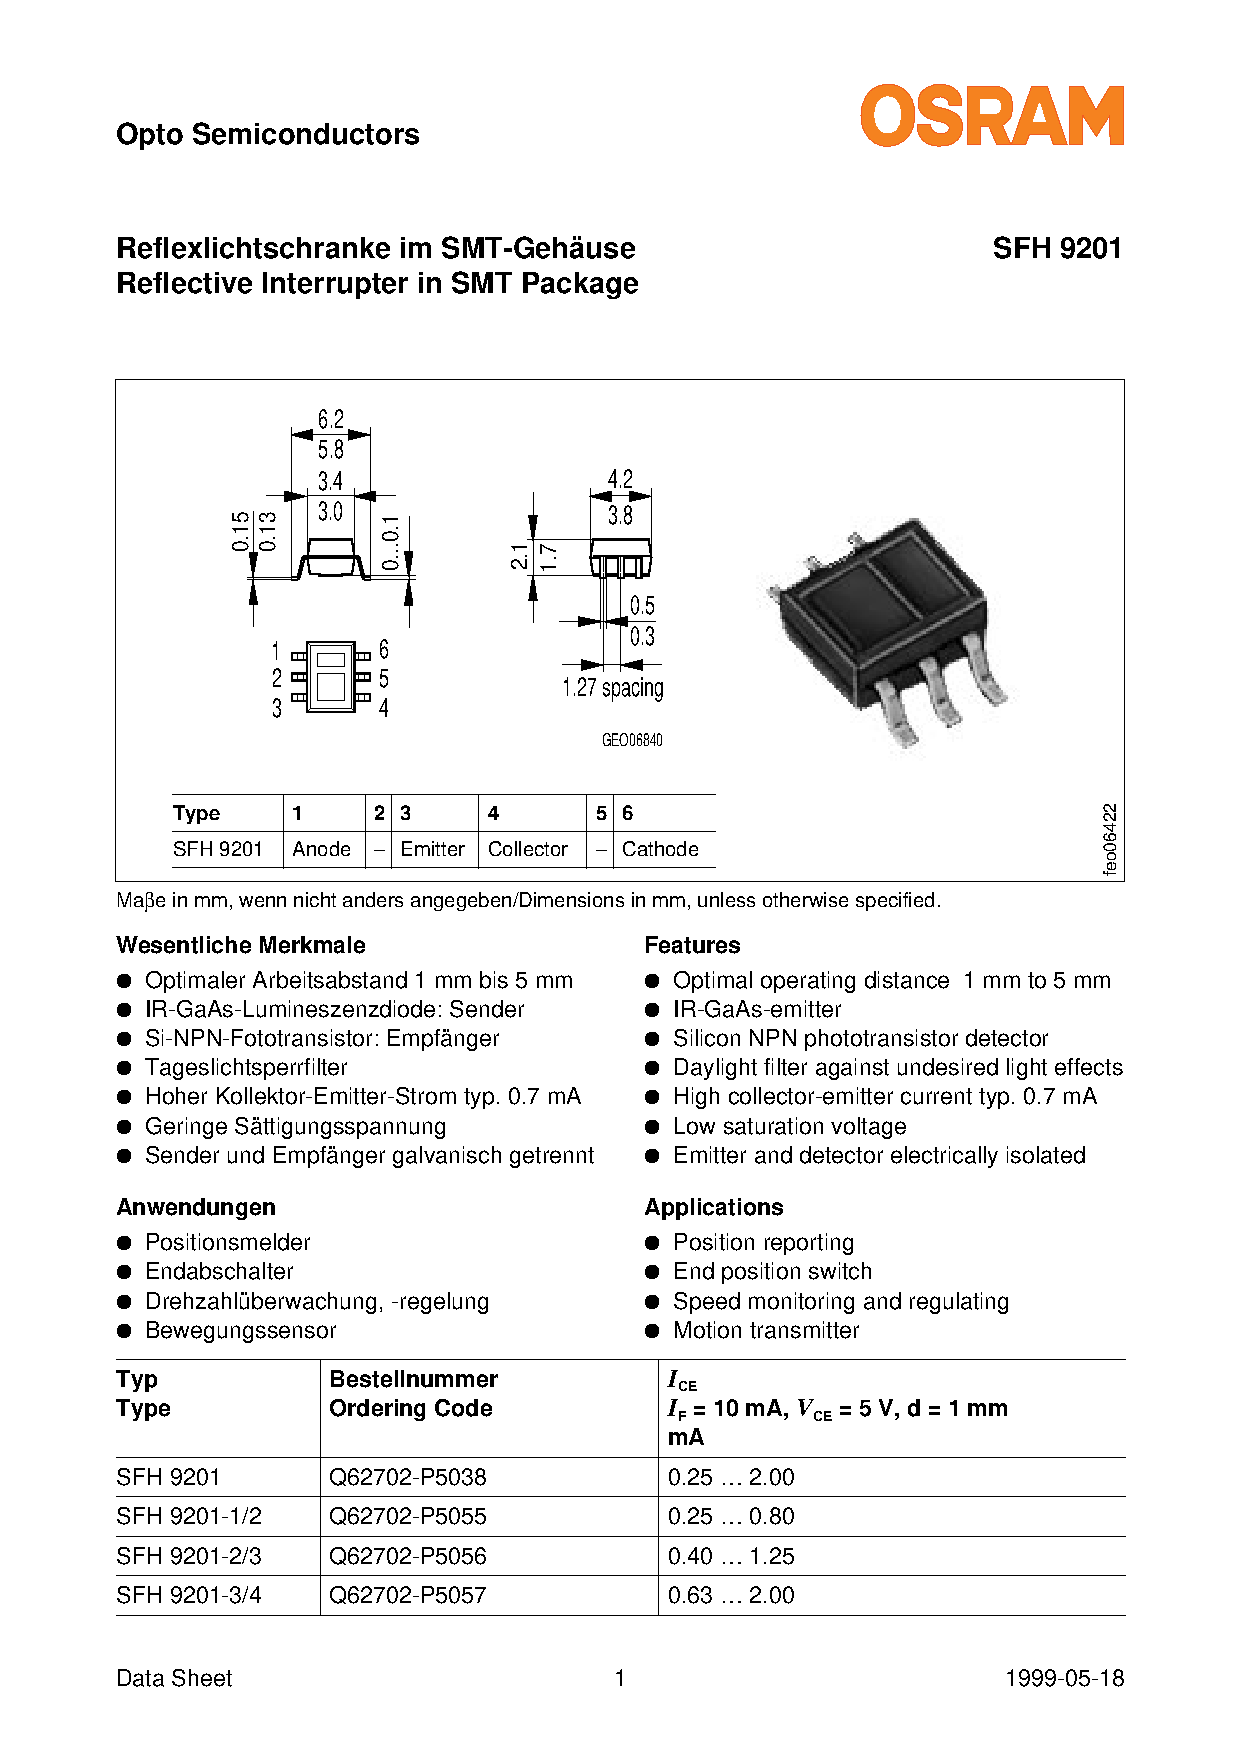
\includepdf[pages={1},pagecommand={\subsection*{Reflexionslichtschranke SFH9201}\label{app:SFH9201}},scale=0.8,frame=true]{Reflexlichtschranke-SFH9201.pdf}
    \includepdf[pages={2-},scale=0.8,frame=true]{Reflexlichtschranke-SFH9201.pdf}
\end{document}
